\PassOptionsToPackage{bookmarks={true}}{hyperref}
\pdfminorversion=4
\documentclass[mathserif,xcolor={dvipsnames,table}]{beamer}
\mode<presentation>{\usetheme{Warsaw}\usecolortheme{crane}}
\usepackage{centernot}
\usepackage{graphicx}
\usepackage{transparent}
\usepackage{geometry}
\usepackage{tikz}
\usetikzlibrary{shadows}
\usepackage[utf8]{inputenc}
\usepackage[english]{babel}
\usepackage[T1]{fontenc}
\usepackage{lmodern}
\usepackage[babel=true]{microtype}
\usepackage{amsmath}
\beamertemplatenavigationsymbolsempty

\title{\textbf{Kernelspace}}
\date{}
\author{CS4803UWS at the\\
Georgia Institute of Technology
}

\begin{document}

{
\setbeamertemplate{background canvas}{%

\includegraphics[width=\paperwidth,height=\paperheight]{images/gt2.jpeg}
}%
\begin{frame}[plain]
\textcolor{white}{
\transparent{0.5}%
\colorbox{black}{\textbf{kernelspace}}
}
\vspace{2.7in}
\\
\hfill
\includegraphics[scale=.25]{images/cc-logo.pdf}

\includegraphics[scale=.25]{images/cc-new.pdf}

\includegraphics[scale=.25]{images/cc-share.pdf}
\textcolor{white}{
\\
\hfill \tiny{CC3.0 share-alike attribution}\\
}
\textcolor{white}{
\hfill \scriptsize{copyright \copyright\ 2013}\\
}
\end{frame}
}

\begin{frame}{Processes}
Process 1\footnote{\tiny{Typically {\tt /sbin/init}; override this with kernel parameter {\tt init=}.}} is launched by the
kernel following initialization. The kernel will panic if {\tt init} cannot be found,
or if process 1 ever terminates. Process 1 is the ultimate ancestor of all userspace
processes, and orphaned processes are reparented to it.
\vfill
On Linux, new processes are launched with {\tt clone(2)}. FreeBSD uses the more
traditional {\tt rfork(2)} interface; GNU libc since 2.3.3 implements {\tt fork(2)}
in terms of {\tt clone(2)}.
\end{frame}

\begin{frame}{Credentials}
%\item[\textbf{PID}] Process ID---positive (kernel processes have PID 0), unique
% integer < {\tt /proc/sys/kernel/pid\_max}. {\tt pid\_t getpid(2) \$\$ /proc/<pid>/stat} (f1).
%\item[\textbf{PPID}] Parent ID---from set of active PIDs {\tt pid\_t getppid(2) \$PPID /proc/<pid>/stat} (f4).
%\item[\textbf{PGID}] Process group ID---unique to each pipeline. Set up by job-controlling shell
% shell. {\tt pid\_t getpgrp(2) N/A /proc/<pid>/stat} (f5).

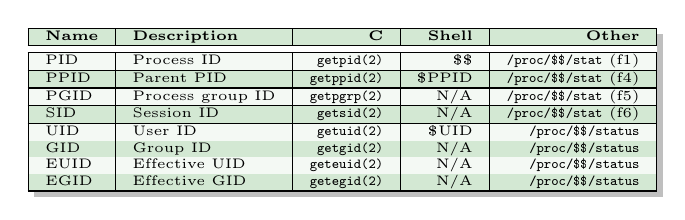
\begin{tikzpicture}
\node[drop shadow,fill=white,inner sep=0pt]
{\rowcolors{1}{ForestGreen!20}{ForestGreen!5}
{\tiny
\begin{tabular}{|l|l|r|r|r|}
\hline
\textbf{Name} & \textbf{Description} & \textbf{C} & \textbf{Shell} & \textbf{Other} \\
\hline\hline
PID & Process ID & {\tt getpid(2)} & \$\$ & {\tt /proc/\$\$/stat} (f1)\\
\hline
PPID & Parent PID & {\tt getppid(2)} & \$PPID & {\tt /proc/\$\$/stat} (f4)\\
\hline
PGID & Process group ID & {\tt getpgrp(2)} & N/A & {\tt /proc/\$\$/stat} (f5)\\
\hline
SID & Session ID & {\tt getsid(2)} & N/A & {\tt /proc/\$\$/stat} (f6)\\
\hline
UID & User ID & {\tt getuid(2)} & \$UID & {\tt /proc/\$\$/status}\\
GID & Group ID & {\tt getgid(2)} & N/A & {\tt /proc/\$\$/status}\\
EUID & Effective UID & {\tt geteuid(2)} & N/A & {\tt /proc/\$\$/status}\\
EGID & Effective GID & {\tt getegid(2)} & N/A & {\tt /proc/\$\$/status}\\
\hline
\end{tabular}%
}
};
\end{tikzpicture}
\end{frame}

\end{document}
